\begin{figure}[t]
    \centering
    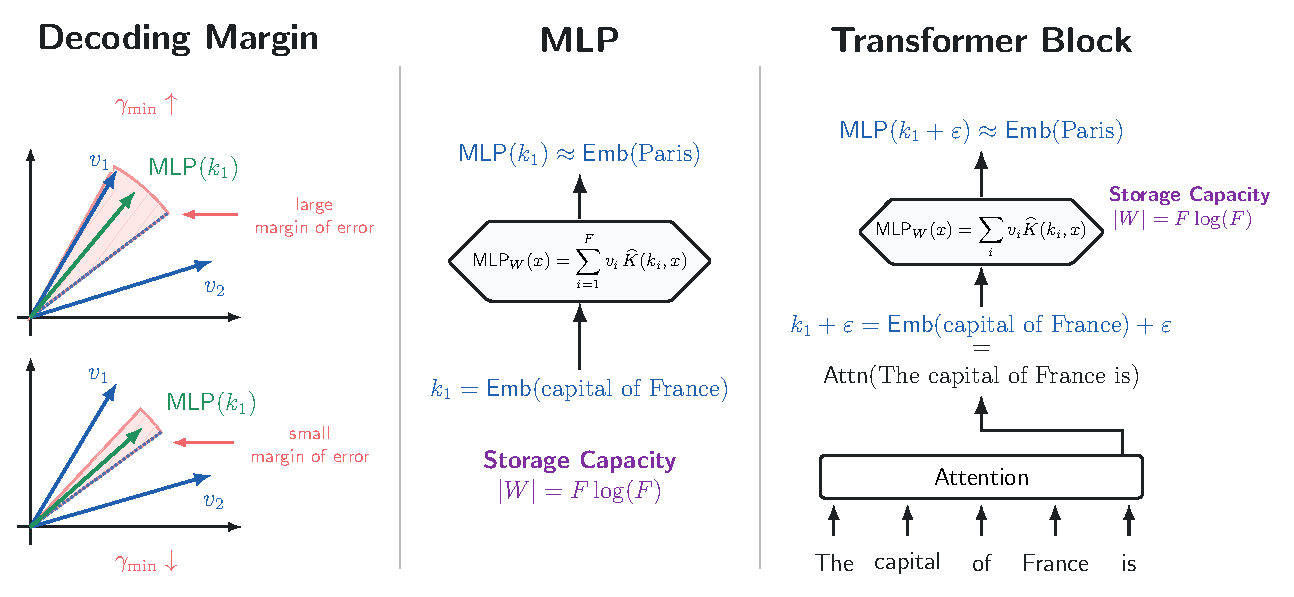
\includegraphics[
        width=\linewidth,
    ]{sections/section_1_intro/figs/banner_fig.pdf}
    \caption{
    \textbf{(A) Decoding margin illustration:} Top plot shows an MLP with large decoding margin, bottom plot with low decoding margin. The MLP with larger decoding margin has a larger ``margin of error'', making it more robust when queried with perturbed versions of $\mathbf{k}_1$. \textbf{(B) MLPs are information-theoretically optimal:} we show that MLPs are Hebbian memories in kernel space and that the storage capacity of MLPs scales at the information-theoretically optimal rate. \textbf{(C) Transformer blocks are information-theoretically optimal:} we show that the storage capacity of Transformer blocks scales at the information-theoretically optimal rate, provided the attention noise remains bounded.
    }
    \label{fig:main-figure}
\end{figure}

